\documentclass[professionalfonts, t, aspectratio=1610]{beamer}
\usepackage{newtxtext,newtxmath}
\usepackage[utf8]{inputenc}
\usepackage[T1]{fontenc}
\usepackage[normalem]{ulem}
\usepackage{wrapfig}

\setbeamertemplate{footline}{
	\hspace*{.5cm}\scriptsize{\insertshorttitle\hspace*{50pt} \hfill\insertframenumber\hspace*{.5cm}}\vspace{9pt}
} 

\title{\textbf{CS636: Internetworking}}
\date[ISPN ’80]{Copyright \textcopyright 2017 by Austin Schwartz \& Eric Theller. All rights reserved}
\author[Comer]{\textbf{Austin Schwartz \& Eric Theller \\ Computer Science \\ Purdue University}}

\usetheme{comer}

\begin{document}

{
  \setbeamertemplate{footline}[text line]{%
    \parbox{\linewidth}{
      \vspace*{-28pt}
      \centering\insertdate
    }
  }
  \begin{frame}
    \titlepage
  \end{frame}
}

\addtocounter{framenumber}{-1}

\setbeamertemplate{footline}[text line]{%
  \parbox{\linewidth}{
    \vspace*{-16pt}
  \hbox{%
    Internetworking With TCP/IP – Course Project
      \insertsectionnavigationhorizontal{.185\paperwidth}{}{}%
   \insertframenumber
      \insertsectionnavigationhorizontal{.4\paperwidth}{}{}%
    2017
    }
    \vspace{0.1cm}
  \hspace*{\fill}%
    \insertdate
  \hspace*{\fill}\vskip2pt%
  }
}

\begin{frame}
\frametitle{ % sorry this is hacky
\bigskip \bigskip \bigskip \bigskip \bigskip \bigskip \\
Module I \\ \bigskip
Introduction\\
And\\
Course Overview} 
\end{frame}

\renewcommand{\baselinestretch}{1.3}
\setbeamercolor{background canvas}{bg=darkcomer}
\begin{frame} 
\frametitle{Austin Schwartz}
\bigskip
\begin{minipage}[0.2\textheight]{\textwidth}
\begin{columns}[T]
\begin{column}{0.6\textwidth}
\begin{itemize}
\item[\textbullet] BS/MS student who has been here forever
\item[\textbullet] Graduating in May
\item[\textbullet] Contributions
  \begin{itemize}
    \item[--] Worked on initial IPv6 + NAT code
    \item[--] Debugging/Printing
    \item[--] Pointed out when things were broken
    \item[--] Made these slides
  \end{itemize}
\item[\textbullet] https://www.austinschwartz.com
\end{itemize}
\end{column}
\begin{column}{0.4\textwidth}
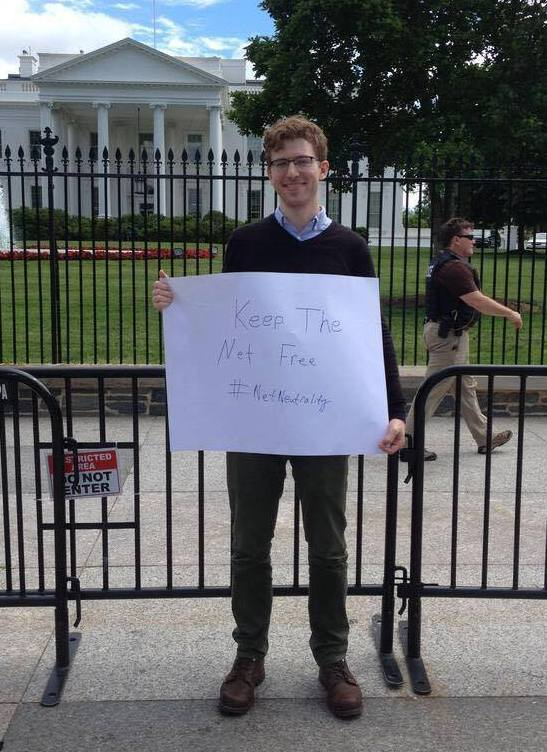
\includegraphics[width=5cm]{austin.jpg}
\end{column}
\end{columns}
\end{minipage}

\end{frame}

\renewcommand{\baselinestretch}{1.3}
\setbeamercolor{background canvas}{bg=darkcomer}
\begin{frame} 
\frametitle{Eric Theller}
\bigskip
\begin{minipage}[0.2\textheight]{\textwidth}
\begin{columns}[T]
\begin{column}{0.6\textwidth}
\begin{itemize}
\item[\textbullet] Undergrad senior
\item[\textbullet] God of VR
\item[\textbullet] Contributions
  \begin{itemize}
    \item[--] Made the shell look like ZSH
    \item[--] Added pretty colors
    \item[--] Made ping/echo
    \item[--] Neighbor Discovery
    \item[--] Made pseudo-forwarding table (if\_of\_ip)
  \end{itemize}
\item[\textbullet] https://www.etheller.com
\end{itemize}
\end{column}
\begin{column}{0.4\textwidth}
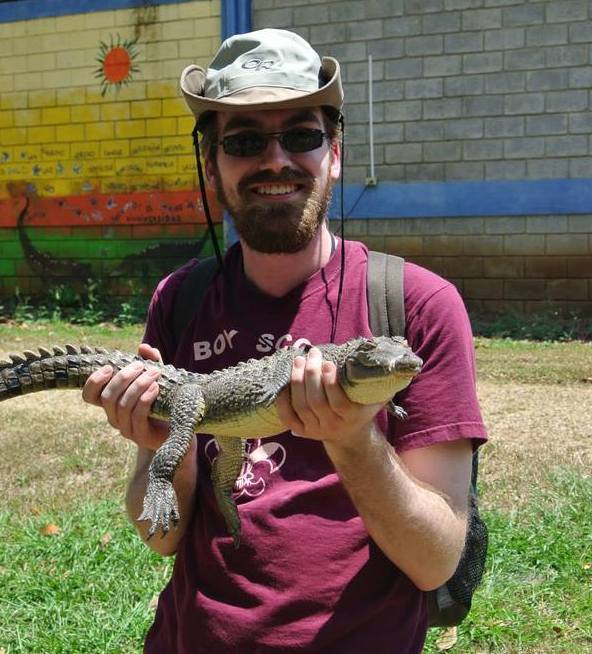
\includegraphics[width=5cm]{eric.jpg}
\end{column}
\end{columns}
\end{minipage}
\end{frame}

\renewcommand{\baselinestretch}{1.3}
\setbeamercolor{background canvas}{bg=darkcomer}
\begin{frame} 
\frametitle{Topic And Scope} 
\bigskip
\bigskip
\bigskip
Internetworking: an overview of concepts, terminology, and technology underlying the TCP/IP Internet protocol suite and the architecture of an internet.
\end{frame}

%\renewcommand{\baselinestretch}{1.3}
%\begin{frame}{You Will Learn}
%\begin{itemize}
%\item[\textbullet] Terminology (including acronyms)
%\item[\textbullet] Concepts and principles
%\begin{itemize}
%  \item[--] The underlying model
%  \item[--] Encapsulation
%  \item[--] End-to-end paradigm
%\end{itemize}
%\item[\textbullet] Naming and addressing
%\item[\textbullet] Functions of protocols including IP, TCP, UDP, SMTP, HTTP, DHCP, and more
%\item[\textbullet] Layering model
%\end{itemize}
%\end{frame}

\renewcommand{\baselinestretch}{1.3}
\begin{frame}{\sout{You Will Learn}\\What We Learned}
\begin{itemize}
\item[\textbullet] Network protocols are complicated
\pause
\item[\textbullet] IPv6 is weird (but some things are really nice!)
\pause
\item[\textbullet] Debugging low level networking code is extremely frustrating.
\pause
\item[\textbullet] You have to have an output queue. You can't just write whenever you want. 
\pause
%  \begin{itemize}
%    \item[--] Committees
%  \end{itemize}
\item[\textbullet] https://en.wikipedia.org/wiki/Design\_by\_committee

\end{itemize}
\end{frame}


\begin{frame}
\frametitle{ % sorry this is hacky
\bigskip \bigskip \bigskip \bigskip \bigskip \bigskip \\
Module II \\ \bigskip
Our Project} 
\end{frame}

\renewcommand{\baselinestretch}{1.3}
\begin{frame}{Our Project}
\begin{itemize}
\item[\textbullet] Neighbor Discovery
\pause
\item[\textbullet] Ping
\pause
\item[\textbullet] NATing
\pause
\item[\textbullet] Pretty colors!
\pause
\item[\textbullet] Bunch of debug shell commands
\pause
\item[\textbullet] Code isn't elegant, but it works
\end{itemize}
\end{frame}

\renewcommand{\baselinestretch}{1.3}
\begin{frame}{Testing}
\begin{itemize}
\item[\checkmark] Othernet h1/h2 -> h0
\pause
\item[\checkmark] h0 <-> xinu front-end
\pause
\item[\checkmark] H0/H1/H2/NAT pinging themselves
\pause
  \begin{itemize}
    \item[--] and loopback address ( ::1)
  \end{itemize}
\item[\checkmark] H1/H2 <-> NAT
\pause
\item[\checkmark] H1/H2 -> Frontend (With hacks)
\pause
\item[$\times$] Pinging on a bad day (IP is best effort)
\end{itemize}
\end{frame}

\renewcommand{\baselinestretch}{1.3}
\begin{frame}{Slides}
\begin{itemize}
\item[\textbullet] Slides available here: https://github.com/lords-of-internetworking/slides
\end{itemize}
\end{frame}



%https://github.com/lords-of-internetworking/slides

\end{document}